
\section{Text Features}
\label{sec:Text Features}
\subsection{Cluster the text features. Can you find meaningful clusters?}
\label{sec:Text Features:a}
 Clustering Text Features
To find meaningful clusters in the annotation text feature space, several dimensionality reduction and clustering strategies were tested. The best results were achieved by first applying t-SNE with a perplexity of 100 to the dataset and then clustering it into 24 clusters using K-Means. \\
To evaluate the quality of these clusters, the most common words in each cluster were analyzed. Clusters dominated by a few semantically consistent keywords (e.g., "dog", "bark", "puppy") were considered well defined, while clusters with a wide range of unrelated terms were considered less consistent.\\
Overall, most clusters represented one or two distinct topics, indicating high cluster quality.


\begin{figure}[h]
  \centering
  \begin{minipage}[b]{0.48\textwidth}
    \centering
    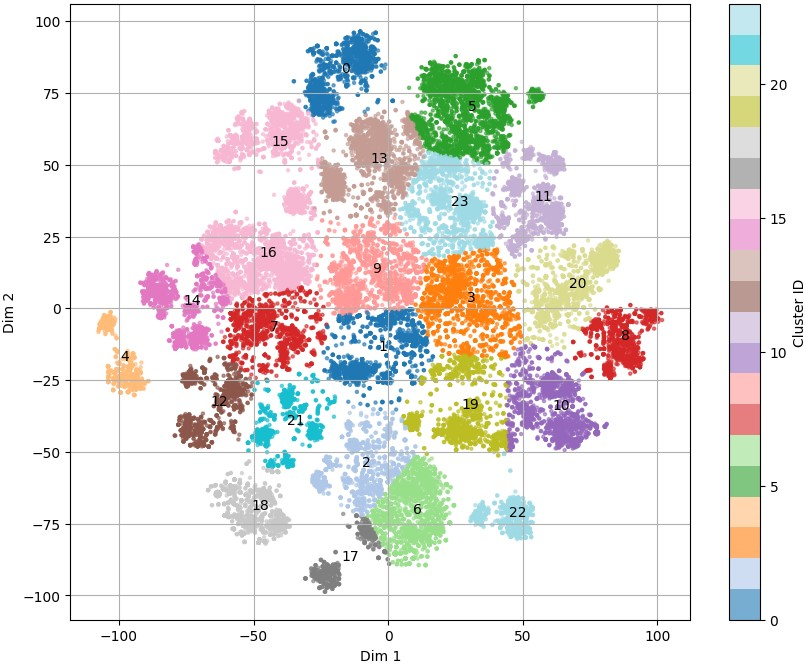
\includegraphics[width=\textwidth]{figs/t-sne_text_clustering.jpg}
    \caption{t-SNE of annotations colored by K-Means clusters}
    \label{fig:image1}
  \end{minipage}
  \hfill
  \begin{minipage}[b]{0.44\textwidth}
    \centering
    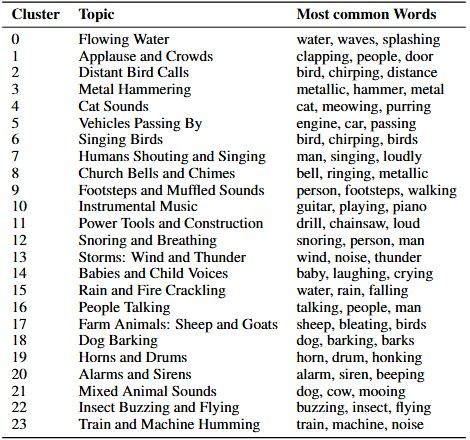
\includegraphics[width=\textwidth]{figs/text_clusters_mainTopics.jpg}
    \caption{Assigned Topics and Top Keywords per Cluster}
    \label{fig:image2}
  \end{minipage}
\end{figure}


\subsection{Design a labeling function1 for classes dog and cat. Do the annotations labeled as dog or cat sounds
form tight clusters in the text and audio feature space?}
\label{sec:Text Features:b}

To evaluate whether semantically similar annotations form tight clusters, labeling functions were created using keyword matching, similar to the ones introduced in the lecture. Simple rule based filters were used to identify dog and cat sounds, relying on a small set of keywords.\\
These functions proved very accurate, identifying large numbers of relevant samples with minimal false positives across the board. The cat related samples clustered almost entirely within a single cluster (cluster 4), showing high cluster purity. Dog related samples appeared primarily in two clusters (clusters 18 and cluster 21), which were spatially adjacent in the 2D t-SNE projection, showing tight clusters for semantically similar topics like cats and dogs.

\begin{figure}[h]
  \centering
  \begin{minipage}[b]{0.49\textwidth}
    \centering
    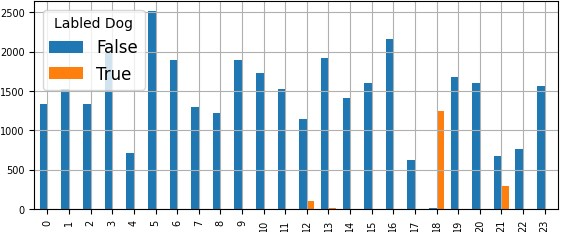
\includegraphics[width=\textwidth]{figs/dog_text_cluster.jpg}
    \caption{Samples labeled dog across text clusters in orange}
    \label{fig:image1}
  \end{minipage}
  \hfill
  \begin{minipage}[b]{0.49\textwidth}
    \centering
    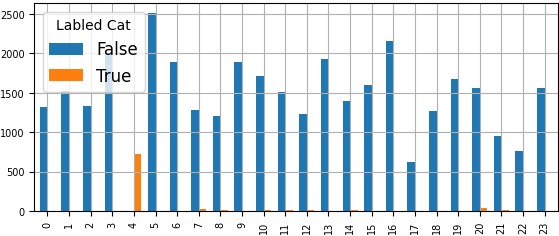
\includegraphics[width=\textwidth]{figs/cat_text_cluster.jpg}
    \caption{Samples labeled cat across text clusters in orange}
    \label{fig:image2}
  \end{minipage}
\end{figure}


\subsection{How well do the audio feature clusters align with text clusters?}
\label{sec:Text Features:c}


To find the relation between audio feature clusters and text clusters, the text clusters were laid over the audio clusters to see if they would fall into a specific cluster. The result varied depending on the cluster, sounds like cat sounds fell almost entirely into a single cluster, while other text clusters, like musical instruments, were spread over multiple clusters.

This is likely because the text space is clustered based on the semantic relation of words, while the audio feature clusters are based on the similarity of sound. For instance, a drone and a violin might end up in the same audio cluster even though their semantic meanings are very different. 
Still, there is a clear connection between the audio feature clusters and text clusters, and many of the clusters align at least in part.

\begin{figure}[h]
  \centering
  \begin{minipage}[b]{0.49\textwidth}
    \centering
    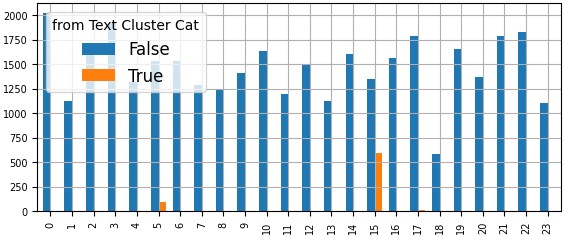
\includegraphics[width=\textwidth]{figs/cat_test_cluster_over_audio_cluster.jpg}
    \caption{Spread of text cluster cat across audio clusters}
    \label{fig:image1}
  \end{minipage}
  \hfill
  \begin{minipage}[b]{0.49\textwidth}
    \centering
    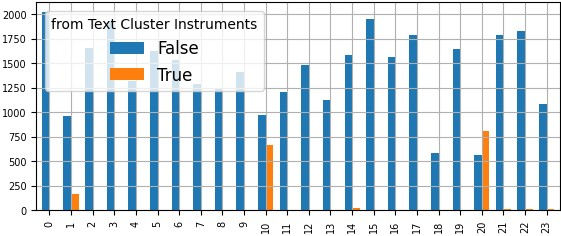
\includegraphics[width=\textwidth]{figs/instruments_test_cluster_over_audio_cluster.jpg}
    \caption{Spread of text cluster instruments across audio clusters}
    \label{fig:image2}
  \end{minipage}
\end{figure}



